%-*-coding: utf-8-*-
\chapter{Теоретическое исследование}

В данной работе было проведено подробное исследование подхода,
представленного в статье~\cite{li2010practical}. В связи с отсутствием
реализации описанного алгоритма в открытом доступе он был реализован с
нуля в полном соответствии с приведённым в статье описанием. В ходе
исследования основное внимание было уделено недостаткам этого
подхода. Были выявлены случаи, в которых описанный алгоритм работает
некорректно. Ниже представлено описание таких случаев, а также
предложены способы решения этих проблем.

\section{Обработка циклов}

В ходе проведённого исследования были выявлены две проблемы базового
алгоритма, связанные с обработкой циклов. Эти проблемы приводят к
ложным срабатываниям. Ниже представлено более подробное описание
недостатков и предложены улучшения, направленные на их устранение.

\subsection{Монотонно изменяющиеся переменные}

\begin{figure}
    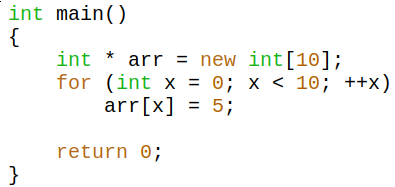
\includegraphics[]{for-trivial.png}
    \caption{Простой цикл: C++}
    \label{fig:for-trivial-cpp}
\end{figure}

\begin{figure}
    \inputTikZ{for-trivial}
    \caption{Простой цикл: SSA форма}
    \label{fig:for-trivial-ssa}
\end{figure}

На рисунке~\ref{fig:for-trivial-cpp} представлен фрагмент C++ кода с
простым циклом, в котором значение переменной $x$ меняется от нуля до
девяти включительно. На рисунке~\ref{fig:for-trivial-ssa} представлена
соответствующая ему SSA форма.

В данном случае алгоритм, описанный в статье~\cite{li2010practical},
будет работать следующим образом. Для проверки корректности записи в
массив будет посчитан диапазон возможных значений переменной $x$ в
месте записи в массив. Для этого сначала будет посчитан диапазон
значений $x$ в месте определения. Изначально в качестве диапазона
будет взят $[\bot, \top]$. Поскольку $x$ выражается как
$\phi$-инструкция, необходимо посчитать диапазон значений $x_1$ в
месте определения $x$ и объединить с $[0, 0]$ (диапазоном значений
второго аргумента). Диапазон значений $x_1$ вычисляется через диапазон
значений $x$ в месте определения $x_1$. Изначально для $x$ был взят
отрезок $[\bot, \top]$, однако в месте определения $x_1$ также будет
применён предикат $x < 10$. Таким образом, диапазон значений $x_1$
будет $[\bot, 10]$. Объединяя его с $[0, 0]$, получаем $[\bot, 10]$ и
для $x$. Это значит, что в данном примере анализатор посчитает, что
$x$ может быть отрицательным, а значит, запись в массив
некорректна. Однако нетрудно видеть, что в действительности это не
так, $x$ не может быть меньше нуля, а запись в массив всегда
корректна. Таким образом, алгоритм выдаёт ложное срабатывание на
данном примере.

Для решения проблемы предлагается использовать дополнительное правило
для вычисления define range. Предположим, что значение $x$ определено
как $\phi(a, b)$, при этом $b = f(x)$. Пусть $f$ удовлетворяет
условию, что последовательность $a, f(a), f(f(a)), \dots$ ---
монотонна (не умаляя общности, предположим, что последовательность
возрастает). Нетрудно видеть, что в таком случае множество возможных
значений $x$ содержится в $\{f^i(a) : i \in [0 .. \inf)\}$ и что все
элементы этого множества не меньше $a$.  Тогда для вычисления define
range $x$ применяется условие $x \geq a$. Примером такой функции $f$
является прибавление или вычитание значения с постоянным знаком.

За счёт использования описанного выше правила в приведённом примере
define range переменной $x$ будет $[0, 10]$, т. к. прибавление единицы
удовлетворяет сформулированному выше условию. Use range в инструкции
записи в массив будет $[0, 9]$. Таким образом, в данном случае удаётся
избежать ложного срабатывания.

\subsection{Обработка предиката «не равно»}

\begin{figure}
    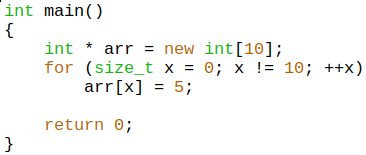
\includegraphics[]{for-ne.png}
    \caption{Цикл с условием «не равно»: C++}
    \label{fig:for-ne-cpp}
\end{figure}

\begin{figure}
    \inputTikZ{for-ne}
    \caption{Цикл с условием «не равно»: SSA форма}
    \label{fig:for-ne-ssa}
\end{figure}

На рисунке~\ref{fig:for-ne-cpp} представлен фрагмент C++ кода с
циклом, аналогичным представленному на
рисунке~\ref{fig:for-trivial-cpp}, но в котором значение счётчика
ограничено с помощью условия «не равно». Такие циклы очень часто
встречаются в программах.  На рисунке~\ref{fig:for-ne-ssa}
представлена соответствующая ему SSA форма.

Подход из статьи~\cite{li2010practical} учитывает предикат $x \neq y$
при вычислении use range переменной $v$ только в том случае, если
равенство $x = y$ выполняется для граничного значения $v$. В таком
случае диапазон значений $v$ сокращается на одно значение. Из-за этого
алгоритм неспособен корректно обрабатывать циклы, в которых значение
счётчика ограничено таким предикатом. В примере на
рисунке~\ref{fig:for-ne-ssa} диапазон значений $x$ без учёта предиката $x \neq
10$ будет $[0, \top]$. Равенство $x = 10$ не соответствует
граничному значению, значит, предикат будет проигнорирован. В
результате алгоритм посчитает, что запись в массив может выйти за
границы, хотя легко видеть, что это не так.

Решение данной проблемы похоже на решение предыдущей проблемы и
заключается в введении дополнительного правила для вычисления use
range. Предположим, что значение $x$ определено как $\phi(a, b)$, при
этом $b = f(x)$. Пусть $f$ снова удовлетворяет условию, что
последовательность $a, f(a), f(f(a)), \dots$ --- монотонна (опять
считаем, что последовательность возрастает). Предположим, что условие
$x \neq y$ всегда выполняется в инструкции $P$, для которой
вычисляется use range переменной $x$. Пусть существует такое $c$, что
$y = f^c(a)$. Нетрудно видеть, что последовательность значений $x$
задаётся как $x_i = f^i(a)$. Из условия существования $c: y = f^c(a)$
и предиката $x \neq y$ следует, что всего может быть не более чем $c$
значений $x$. Из свойства функции $f$ следует, что $x < f^c(a) =
y$. Таким образом, при вычислении use range применяется предикат
$x < y$.

В примере на рисунке~\ref{fig:for-ne-ssa} $f(x) = x + 1$, $y = 10$,
$a = 0$, $c = 10$. Таким образом, анализатор способен вывести, что
$x < 10$, за счёт чего обращение к массиву будет обработано корректно.

\FloatBarrier

\section{Учёт предикатов}

\begin{figure}
    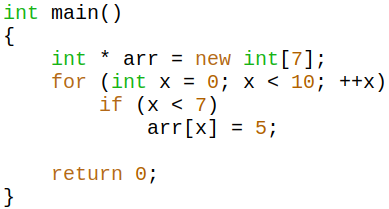
\includegraphics[]{predicates-improvement.png}
    \caption{Цикл с дополнительным условием внутри: C++}
    \label{fig:predicates-improvement-cpp}
\end{figure}

\begin{figure}
    \inputTikZ{predicates-improvement}
    \caption{Цикл с дополнительным условием внутри: SSA форма}
    \label{fig:predicates-improvement-ssa}
\end{figure}

В цикле, представленном на
рисунке~\ref{fig:predicates-improvement-cpp}, значение переменной $x$,
использующейся как индекс при записи в массив, дополнительно
ограничено числом $7$. Таким образом, значение счётчика цикла
находится в диапазоне $[0, 9]$, однако значение индекса не превышает
$7$. Программа в SSA форме представлена на
рисунке~\ref{fig:predicates-improvement-ssa}.

Проблема подхода~\cite{li2010practical} состоит в правиле,
определяющем, какие предикаты должны учитываться при вычислении use
range переменной $v$ в инструкции $P$. Во-первых, условный переход,
использующий предикат, должен доминировать инструкцию $P$, то есть все
пути из входа в функцию в $P$ должны проходить через
предикат. Во-вторых, $P$ должна быть достижима только из одного
потомка условного перехода. Однако, как нетрудно видеть из
рисунка~\ref{fig:predicates-improvement-ssa}, в данном случае
инструкция записи в массив достижима из обоих потомков условного
перехода. Это приводит к тому, что условие $x < 7$ не применяется для
вычисления use range $x$ в месте записи в массив, из-за чего
анализатор выдаёт несуществующую ошибку.

Описанная проблема может быть решена модификацией второго правила,
определяющего, должен ли учитываться предикат при вычислении use
range. Модифицированное правило ослабляет требование, что инструкция
$P$ должна быть достижима только из одного потомка условного перехода,
использующего предикат. Ослабленное требование заключается в том, что
должен быть ровно один потомок $S$ условного перехода $C$, такой что
$P$ достижима из $C$, игнорируя все рёбра из $C$, кроме
$C \rightarrow S$. В таком случае условие, соответствующее переходу в
$S$, считается выполненым.

Покажем, что предложенная модификация сохраняет
корректность. Рассмотрим произвольный путь в инструкцию $P$. По
первому правилу $P$ доминируется $C$, а значит, путь обязан пройти
через $C$. Рассмотрим последнее ребро на этом пути, исходящее из
$C$. Пусть это ребро $C \rightarrow T$. Если $T = S$, значит, условие,
соответствующее переходу в $S$, выполнено, что и требовалось
доказать. Если же $T \neq S$, то путь в $P$ проходит по другому ребру
из $C$, а значит, предположение о том, что ребро $C \rightarrow T$
является последним на пути, неверно.

При использовании модифицированного правила предикат $x < 7$ будет
учтён в месте записи в массив, т. к. из вершины $x_1 = x + 1$ нет
пути, не проходящего по ребру, соответствующему условию $x < 7$. Таким
образом, предложенная модификация позволяет избавиться от ложного
срабатывания в приведённом примере, при этом сохраняя общую
корректность анализа.

\FloatBarrier

\section{Межпроцедурный анализ}

В статье~\cite{li2010practical} описывается лишь алгоритм без
межпроцедурного анализа. Каждая функция анализируется независимо,
информация о возможных значениях аргументов игнорируется. Каждый
аргумент рассматривается точно так же, как и любое значение,
приходящее извне. На практике программы обычно состоят из большого
числа маленьких функций, и анализа одной изолированной функции
недостаточно, чтобы точно определить, всегда ли обращение к массиву
корректно.

В данной работе анализ был расширен до межпроцедурного. В целом
известно два общих подхода к межпроцедурному анализу: в одном подходе
при анализе вызывающей стороны определяются возможные значения
аргументов и используются для анализа вызываемой функции, в другом
подходе при анализе вызываемой функции определяются условия, которым
должны соответствовать аргументы, и проверяются при непосредственном
вызове. В данной работе используется второй вариант. Основная идея
описана в статье~\cite{xie2003archer}. Функции анализируются в порядке
топологической сортировки: от вызываемой к вызывающей. Если в графе
вызовов есть цикл (рекурсия), то топологическая сортировка
неопределена, и в таком случае цикл разрывается в случайных
местах. Также вводится понятие триггера, который задаёт условие,
влияющее на факт выхода за пределы массива. При анализе вызываемой
функции формируется множество триггеров. При анализе вызова функции
проверяется выполнимость каждого триггера.

\subsection{Триггеры}

Триггер задаётся упорядоченной парой символьных выражений $e_1$ и
$e_2$. Оба выражения должны состоять только из констант и аргументов
функции (включая их афинные преобразования). Смысл триггера в том, что
если $e_1 \prec e_2$, то это приведёт к выходу за пределы
массива. Также триггер должен хранить внутри себя инструкцию, в
которой может произойти выход за пределы массива, чтобы при его
срабатывании можно было понять, в каком месте случится ошибка.

\begin{figure}
    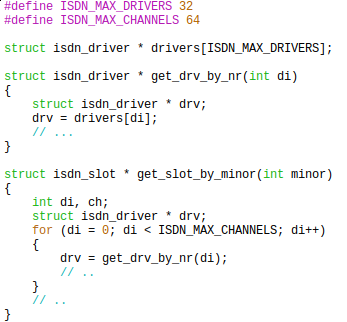
\includegraphics[]{archer-linux.png}
    \caption{Межпроцедурный анализ}
    \label{fig:archer-linux}
\end{figure}

Для иллюстрации рассмотрим упрощённый фрагмент кода из ядра Линукс
версии 2.5.53, представленный на рисунке~\ref{fig:archer-linux}. В
данном примере функция \texttt{get\_slot\_by\_minor} вызывает функцию
\texttt{get\_drv\_by\_nr}. При анализе \texttt{get\_drv\_by\_nr} будет произведено
построение триггеров для этой функции. Затем эти триггеры будут
проверены при анализе \texttt{get\_slot\_by\_minor} (она будет анализирована
после \texttt{get\_drv\_by\_nr}, поскольку функции анализируются в порядке
топологической сортировки). Нетрудно видеть, что в данном случае выход
за пределы массива в функции \texttt{get\_drv\_by\_nr} может произойти тогда
и только тогда, когда $ISDN\_MAX\_DRIVERS \leq di \vee di \leq
-1$. Таким образом, для функции должно быть построено два триггера,
соответствующих этим неравенствам. В функции \texttt{get\_slot\_by\_minor}
происходит вызов \texttt{get\_drv\_by\_nr}, и в месте вызова можно расчитать
диапазон возможных значений аргумента, передаваемого в
\texttt{get\_slot\_by\_minor}. За счёт этого можно вывести, что один из
триггеров выполняется в месте вызова, а значит, в программе есть
ошибка.

Использование триггеров позволяет учесть информацию о значениях
аргументов функций, а также о завимостях между этими аргументами. Ниже
представлено более подробное описание использования триггеров.

\subsection{Построение триггеров}

Построение триггеров происходит при определении корректности доступа к
массиву в тех случаях, когда одно или несколько рассматриваемых
символьных значений зависят от аргументов функции. Как уже было
сказано в первой главе, выход за пределы массива размера $n$ при
обращении по индексу $index$ (инструкция $P$) фиксируется, если
$S_{n, P}^{max} \prec S_{index, P}^{max}$ или
$S_{index, P}^{min} \prec -1$. Таким образом, для проверки
используются диапазоны $n$ и $index$. Если $S_{n, P}^{max}$ или
$S_{index, P}^{max}$ зависит от аргумента функции, то их сравнение в
общем случае невозможно. В таком случае для функции добавляется
триггер $S_{n, P}^{max} \prec S_{index, P}^{max}$, хранящий также
инструкцию $P$. Выполнение этого триггера означает выход за пределы
массива в результате исполнения инструкции $P$. Аналогично
обрабатывается условие $S_{index, P}^{min} \prec -1$. В результате
обработки функции все сгенерированные триггеры сохраняются в
глобальном контексте анализатора для дальнейшей проверки в месте
вызова. Если при проверке был сгенерирован хотя бы один триггер, то
выход за пределы массива не фиксируется, а проверка откладывается для
вызывающей стороны.

Вернёмся к примеру, представленному на
рисунке~\ref{fig:archer-linux}. При анализе обращения к массиву
$drivers$ внутри функции \texttt{get\_drv\_by\_nr} (назовём эту инструкцию
$P$) необходимо проверить два условия: $32 \prec S_{di, P}^{max}$ и
$S_{di, P}^{min} \prec -1$. Поскольку $di$ является аргументом
функции, оба условия приведут к созданию триггера для рассматриваемой
функции, ассоциированных с инструкцией $P$. Триггеры будут сохранены и
проверены во время анализа функции \texttt{get\_slot\_by\_minor}.

Описанное правило применяется в тех случаях, когда рассматриваемые
символьные выражения зависят только от констант и аргументов
функции. Точно так же обрабатываются случаи, когда символьное
выражение задаётся функцией от нескольких аргументов. Например, если
бы функция принимала также аргумент $si$, а обращение происходило по
индексу $2 * si - di$, то такое символьное выражение тоже привело бы к
созданию триггера. За счёт этого учитываются зависимости между
аргументами, которые нередко имеют место в сложных функциях.

\subsection{Проверка триггеров}

При анализе инструкции вызова функции происходит проверка выполнимости
триггеров, сохранённых для этой функции. Напомним, что триггер состоит
из двух символьных выражений, в которых могут присутствовать аргументы
вызываемой функции. Каждому аргументу вызываемой функции соответствует
какое-то значение из вызывающей функции. Для каждого такого значения
рассчитывается диапазон значений в месте вызова функции (use
range). Таким образом, в общем случае символьным выражениям $e_1$ и
$e_2$, сравниваемым для проверки триггера, соответствуют символьные
отрезки $r_1$ и $r_2$. После вычисления $r_1$ и $r_2$ проверка
триггера происходит аналогично проверке выходу за пределы массива в
простом случае. Если $r_1^{max} \prec r_2^{min}$, то триггер всегда
выполняется, и в таком случае фиксируется ошибка. Если
$r_2^{max} \prec r_1^{min} + 1$, то ошибки точно нет. В противном
случае ошибка потенциально может произойти, но не точно. По умолчанию
в спорных ситуациях ошибка не фиксируется для избежания слишком
большого числа ложных срабатываний.

В примере на рисунке~\ref{fig:archer-linux} при анализе вызова функции
\texttt{get\_drv\_by\_nr} из функции \texttt{get\_slot\_by\_minor} проверяются два
триггера, построенные при анализе \texttt{get\_drv\_by\_nr}:
$32 \prec S_{di, call}^{max}$ и $S_{di, call}^{min} \prec -1$, где
$di$ является аргументом \texttt{get\_drv\_by\_nr}, а $call$ --- инструкция
вызова функции. В данном случае диапазон $S_{di, call}$ будет вычислен
как $[0, 64]$. В результате будет выполнено условие первого триггера,
что приведёт к сообщению об ошибке. За счёт хранения инструкции, в
которой происходит обращение к массиву, вместе с триггером анализатор
сможет сообщить и место вызова функции, и место внутри функции, в
котором случается ошибка.

\FloatBarrier

\chapterconclusion

В главе 2 представлены результаты исследования алгоритма,
описанного в статье~\cite{li2010practical}. В ходе исследования были
выявлены различные недостатки алгоритма, которым было уделено внимание
в данной работе. Показаны примеры кода, когда алгоритм работает
некорректно, предложены модификации исходного алгоритма, направленные
на устранение выявленных проблем. Доказана корректность предложенных
модификаций.

Одним из наиболее значимых улучшений является использование
межпроцедурного анализа, что крайне важно для анализа промышленных
программ. Предложенный подход базируется на идеях, использованных в
статье~\cite{xie2003archer}, однако адаптирован для алгоритма из
статьи~\cite{li2010practical}.
